\documentclass[a4paper, 11pt, twocolumn]{article}
\usepackage[top=2cm, bottom=3cm, left = 2cm, right = 2cm]{geometry} 
\geometry{a4paper} 
\usepackage{textcomp}
\usepackage{graphicx} 
\usepackage{amsmath,amssymb}  
\usepackage{bm}  
\usepackage{memhfixc} 
\usepackage{fancyhdr}
\usepackage{enumerate}
\usepackage{float}
\usepackage{xcolor}
\usepackage{booktabs}
\usepackage{algpseudocode}
\usepackage{algorithm}
\usepackage{varwidth}
\usepackage{listings}
\usepackage[framed]{ntheorem}
\usepackage{hyperref}
\usepackage{authblk}
\pagestyle{fancy}
\setlength{\headheight}{14pt}
%\addtolength{\topmargin}{-2pt}
\theoremstyle{nonumberplain}

\newtheorem{definition}{Definition}

\algdef{SE}{Begin}{End}{\textbf{begin}}{\textbf{end}}

\definecolor{commentsColor}{rgb}{0.497495, 0.497587, 0.497464}
\definecolor{keywordsColor}{rgb}{0.000000, 0.000000, 0.635294}
\definecolor{stringColor}{rgb}{0.558215, 0.000000, 0.135316}

\lstset{ %
  backgroundcolor=\color{white},   % choose the background color; you must add \usepackage{color} or \usepackage{xcolor}
  basicstyle=\footnotesize,        % the size of the fonts that are used for the code
  breakatwhitespace=false,         % sets if automatic breaks should only happen at whitespace
  breaklines=true,                 % sets automatic line breaking
  captionpos=b,                    % sets the caption-position to bottom
  commentstyle=\color{commentsColor}\textit,    % comment style
  deletekeywords={...},            % if you want to delete keywords from the given language
  extendedchars=true,              % lets you use non-ASCII characters; for 8-bits encodings only, does not work with UTF-8
  frame=tb,	                   	   % adds a frame around the code
  keepspaces=true,                 % keeps spaces in text, useful for keeping indentation of code (possibly needs columns=flexible)
  keywordstyle=\color{keywordsColor}\bfseries,       % keyword style
  otherkeywords={*,...},           % if you want to add more keywords to the set
  numbers=left,                    % where to put the line-numbers; possible values are (none, left, right)
  numbersep=5pt,                   % how far the line-numbers are from the code
  numberstyle=\tiny\color{commentsColor}, % the style that is used for the line-numbers
  rulecolor=\color{black},         % if not set, the frame-color may be changed on line-breaks within not-black text (e.g. comments (green here))
  showspaces=false,                % show spaces everywhere adding particular underscores; it overrides 'showstringspaces'
  showstringspaces=false,          % underline spaces within strings only
  showtabs=false,                  % show tabs within strings adding particular underscores
  stepnumber=1,                    % the step between two line-numbers. If it's 1, each line will be numbered
  stringstyle=\color{stringColor}, % string literal style
  tabsize=2,	                   % sets default tabsize to 2 spaces
  title=\lstname,                  % show the filename of files included with \lstinputlisting; also try caption instead of title
  columns=fixed                    % Using fixed column width (for e.g. nice alignment)
}

\title{Shared Memory Process Communication in VMs and Containers Host}

\author{Hossein Afkar\\ \href{mailto:hossein.afkar@ut.ac.ir}{hossein.afkar@ut.ac.ir}}
\affil{Department of Computer Science, University Of Tehran}

%\date{}

\begin{document}
\maketitle
% \tableofcontents

\section{Introduction}
Inter-process communication is a very important part of os and infrastructure
design. To utilize newer design methodologies like micro-kernel and
exo-kernel we need to be aware of inter-process communication. \\
Cloud and edge infrastructure also need ways to ease the communication
between their tenants. VMs and containers are a common tenant of the
distributed systems which makes their communication more important for us as
an operating systems designer. With the rise of Industry 4.0 and 
distributed real-time systems, it has become apparent to us that a deterministic
communication method is of utmost importance to a real-time system
designer. \\
In this report, we try to explore the area surrounding real-time systems and
their communication. By exploring ideas and new designs surrounding virtual
machines and containers Our goal is to study and propose a design based on our
findings and papers studied in the advanced operating systems course.
\section{Ideas and Design}
In this section, we will try to investigate the ideas surrounding virtualization
and inter-process communication. To achieve an effective and
deterministic approach to the communication between the virtualized world we
should be aware of the tools and standards present to help us achieve our
goal. \\
Our goals are indicated as follows:
\begin{itemize}
    \item Consolidate various ECUs used in Industry 4.0.
    \item Tackle communications between units present in the same
        host that were separated before.
    \item Fast and not marshaled solution for local tenants.
    \item No contention on the memory bus.
    \item No contention on locks.
    \item Bound the memory access latency.
\end{itemize}
To achieve our goals we will try to investigate each part according to
its features and try to understand each part carefully before proposing our
design.
\subsection{Industry 4.0 and real-time systems}
Industry 4.0 also known as the Forth industrial revolution revolves around
the notion of integrating the manufacturing landscape with advanced
technologies and real-time systems. \\
Real-time systems play a critical role in the formation of Industry 4.0.
These systems enable the factory to collect, analyze, and utilize the collected
data in real-time to optimize a process, enhance productivity, and drive
innovation. \\
Virtualization plays a crucial role in Industry 4.0 by enabling the efficient
utilization of resources, enhancing flexibility, and facilitating the
integration of diverse systems and technologies. \\
In Industry 4.0, virtualization allows for the creation of virtual machines
(VMs) or containers that encapsulate entire operating systems or specific
applications, respectively. This enables the consolidation of multiple
virtual instances on a single physical server, optimizing resource
utilization and reducing hardware costs. \\
Moreover, virtualization provides the flexibility to scale resources up or
down based on demand, allowing for dynamic allocation of computing power and
storage. By abstracting the underlying hardware, virtualization also
simplifies the integration of different systems and technologies,
enabling seamless communication and interoperability. \\
Overall, virtualization is a key enabler of the agility, scalability,
and efficiency required in the complex and interconnected
manufacturing systems of Industry 4.0. \\
One of the main challenges in the virtualization world is crossing the
isolation barrier for communication. This makes effective and deterministic
communication important for real-time systems design.
\subsection{Virtualization Techniques}
Virtualization techniques play an important role in providing the isolation
of the resources required for real-time systems. \\
Virtualization provides us with several benefits such as:
\begin{itemize}
    \item Scalability and Flexibility.
    \item Improved Disaster Recovery and Business Continuity.
    \item Simplified Management and Deployment.
\end{itemize}
The benefits provided by virtualization techniques are vast and the benefits stated
above are good to have in an environment like Industry 4.0 where security,
scalability, and flexibility are of utmost importance. \\
In the next subsection, we will try to explore and compare virtual machines and
containers.
\subsubsection{Virtual Machines}
Virtual machines are the first-class tenant of the virtualization world.
As stated in the name virtual machines try to emulate a machine. \\
Virtual machines are an efficient, isolated duplicate of a real computer
machine. Virtual Machines are used when the need for isolation is bigger than
anything else. Virtual machines provide ironclad isolation, therefore
communication in the VM boundary is harder than average inter-process
communication. \\
Most ways involving different VMs communication is based on network or
network devices. The network is a battle-tested method of communication in virtual
machines, but its nondeterministic nature and overhead make it an unviable choice 
for inter-host communications. In this report, we choose to invest in shared
memory methods. Shared memory regions enable fast transmission of data without
the overhead of marshaling between different VMs in the same host. \\
Enabling shared memory regions is a hard job considering the isolation of
resources done in virtual machines. Page tables and virtual machines
monitor can not do a good job of enabling shared memory regions because of
added complexity and attack surface in the operating system. The best way is
to use a pseudo device to reach our goals. This device can be a disk drive
that makes the aforementioned memory regions available to the whole host. \\
The approach used by the Xen hypervisor can be used to emulate such devices.
One of the standardized ways of doing so is using the VirtIO block device.
VirtIO is a virtualization standard that provides a framework for efficient
and high-performance communication between virtual machines and
their host systems. It defines a set of device drivers and a common interface
that allows VMs to interact with virtual devices, such as network adapters
and storage controllers, in a standardized and efficient manner. \\
VirtIO leverages paravirtualization techniques to minimize the overhead
of virtualization and maximize performance. By using a common interface,
Virtio enables seamless interoperability between different hypervisors and
guest operating systems, making it easier to migrate VMs across different
virtualization platforms. Overall, Virtio plays a critical role in enhancing
the performance, flexibility, and compatibility of virtualized environments.
VirtIO uses ring buffers to simplify the producer and consumer problems.
A similar approach (ring buffer) was used in Xen device drivers.
% VirtIO figure may do good.
\begin{figure}[H]
    \center
    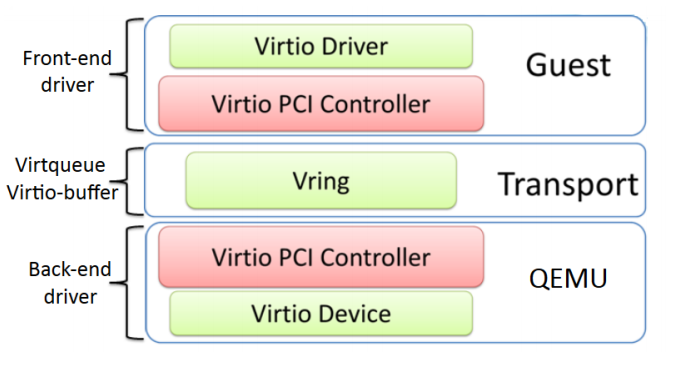
\includegraphics[width=0.5\textwidth]{virtio.png}
    \caption{VirtIO Architecture In QEMU hypervisor}
    \label{virtio}
\end{figure}
\subsubsection{Containers}
Container technology is a lightweight virtualization method that allows for
the efficient and isolated execution of applications. Containers package
an application and its dependencies into a single, portable unit,
enabling consistent deployment across different environments.
They leverage the host operating system, sharing its kernel and
resources, which results in faster startup times and lower resource
overhead compared to traditional virtual machines. Containers provide
a high level of scalability, allowing for the rapid deployment and
scaling of applications, making them well-suited for modern, dynamic,
and cloud-native environments. \\
Container runtimes consist of containerd and lxc. the choice of the container
runtime is irrelevant to us because container runtimes are a wrapper over
cgroups and namespaces. containers become possible by using the aforementioned
features in the Linux kernel. In this report, we focus on the cgroups and
namespaces for the management of containers. Containers existed well before the
Linux implementation of cgroups and namespaces. FreeBSD jail mechanism employs
a similar idea to chroot and Linux control groups that make the containers
possible in BSD-based systems. \\
Cgroups or control groups are a Linux feature that provides us with process
control and grouping. By using cgroups we can group processes and apply rules
and isolation upon them. Process isolation is done by cgroups. \\
Linux namespace API helps us partition kernel resources like unique ids and
inter-process communications. Isolation is provided through cgroups and
namespaces. Container isolation is weaker than the one seen in the virtual
machines. One example is that the CPU limits enforced on the process groups
may not behave as strongly as the ones in virtual machines. \\
Container communications like their virtual machine counterparts
mostly happen on the network layer. Containers mostly communicate using
RPC over the network. Shared memory communication is not common in the container
world but is possible. All we have to do is to tell the container runtime
to create a shared namespace for the IPC subsystem. \\
Another notion that is developing in recent years is the MicroVM design.
MicroVM states that most of the whole system emulation is unnecessary. System
components like ACPI calls and PCI bus should not be present when our vm does
not need it. So the idea is to make a minimal os and virtual machines just to
run programs and remove overheads. This idea is used in AWS lambda with
FireCracker virtual machine monitor. QEMU recently added this feature with
\textit{-M microvm} machine type.
MicroVM uses VirtIO for device declaration, effectively reducing device drivers'
footprint.
\subsubsection{Containers vs VMs}
Container technology is a lightweight virtualization method that allows for
the efficient and isolated execution of applications.
Containers package an application and its dependencies into a single,
portable unit, enabling consistent deployment across different environments.
They leverage the host operating system, sharing its kernel and resources,
which results in faster startup times and lower resource overhead compared to
traditional virtual machines. Containers provide a high level of scalability,
allowing for the rapid deployment and scaling of applications, making them
well-suited for modern, dynamic, and cloud-native environments. Additionally,
containers offer enhanced flexibility, as they can be easily moved,
replicated, and managed using container orchestration platforms like
Kubernetes.
\begin{table}[H]
    \centering
    \begin{tabular}{|p{0.2\textwidth}|p{0.2\textwidth}|} \hline
        Virtual Machines & Containers \\ \hline
        Kernel and various resources are virtualized, with High overhead
        & Kernel is shared as a resource. Lowers the overhead \\ \hline
        High isolation & Subpar resource isolation \\ \hline
        Startup time is kernel and userland & Only userland \\ \hline
        Does not rely on host os & Relies on host os \\ \hline
        Hypervisor managed & Kernel managed \\ \hline
    \end{tabular}
    \caption{Comparing Containers And Virtual Machines}
\end{table}

\subsection{MemGuard: Memory Bandwidth Control}
Memory bandwidth is a highly varied resource in multi-core systems.
Access times of a memory request are dependent on the location of the access
and the state of the DRAM chip. There is also the inter-core dependency of the
memory accesses. \\
The memory controller schedules the accesses to maximize the overall DRAM
throughput.
As real-time and embedded applications become more memory intensive, to
guarantee performance isolation we should allocate the memory bandwidth
among the different cores. MemGuard \cite{memguard} approach is related to
the memory bandwidth. By reading the performance counters of each core they
succeeded in isolating the memory performance. Memory performance isolation is
a very important trait for mixed-critical systems and real-time applications.
To control the bandwidth of an application MemGuard paper does
the following approach:
\begin{itemize}
    \item Program Performance monitor counter to overflow on a certain value
        known as the core budget.
    \item If the core is over the budget dequeue all tasks from the run queue.
    \item If there is an Unused budget from the other cores split the budget for
        the core that is surpassing its budget.
\end{itemize}
MemGuard algorithms are more elaborate than the steps stated above. For
more information refer to the \cite{memguard}.

\subsection{io\_uring: Asynchronous system calls}
io\_uring is a mechanism for performing asynchronous I/O. Classic Unix I/O has
always been inherently synchronous. As far as an application is concerned,
an operation is complete once a system call like read() or write() returns,
even if some processing may continue behind its back. In the Linux world,
this gap was filled with asynchronous I/O subsystems. The POSIX specifies
aio\_read and aio\_write but the performance is poor and the implementation
is suboptimal. Also, This subsystem has been deprecated in favor of io\_uring.
io\_uring consists of a ring buffer to simplify single consumer and single
producer. This approach is already used in the network device drivers and
Xen hypervisor.
\begin{figure}[H]
    \center
    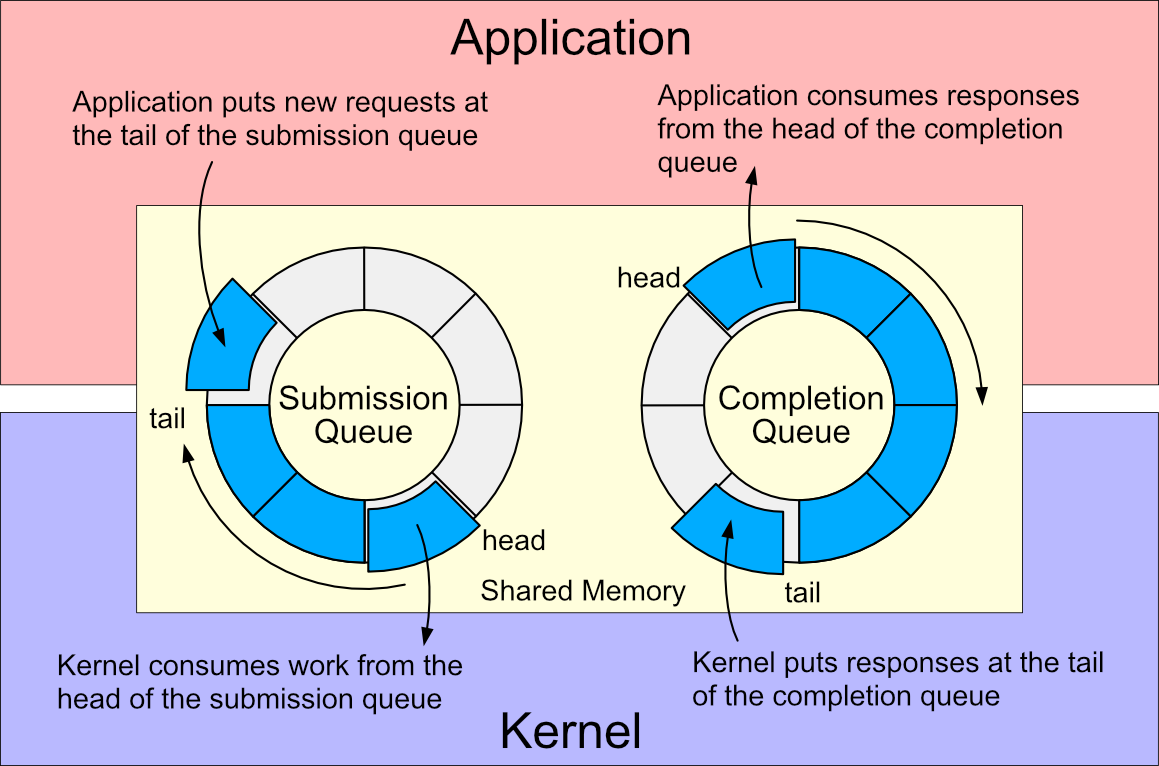
\includegraphics[width=0.5\textwidth]{uring.png}
    \caption{io\_uring Inner Workings Showing Two Ring Buffer}
    \label{uring}
\end{figure}
io\_uring simplifies most I/O applications. By removing the overhead of
multiple border crossings, we can implement most of our functionality in
the kernel without the fear of losing performance. But we must also
keep in mind with io\_uring we are following the monolithic kernel
philosophy. Overall io\_uring presents us with a way to remove the overhead
of the blocking system calls and is moving forward in the Linux kernel
development.

\subsection{Cache Coloring}
Cache coloring is a technique used in computer systems to optimize memory
performance by reducing conflicts in the cache. In a computer system,
the cache is a small, fast memory that stores frequently accessed data.
When a program accesses data, it is first checked in the cache.
If the data is found in the cache, it is called a cache hit, resulting in
faster access. However, if the data is not found in the cache,
it is called a cache miss, and the data needs to be fetched
from the main memory, resulting in slower access. \\
Cache coloring aims to minimize cache conflicts by assigning
different memory pages to different cache sets. Cache sets are subsets of
the cache that can hold a certain number of memory pages.
By assigning different memory pages to different cache sets,
the likelihood of two memory pages that are frequently
accessed together being assigned to the same cache set is
reduced. This reduces cache conflicts and improves cache hit rates,
leading to better memory performance. \\
Cache coloring is particularly useful in systems with direct-mapped caches,
where each memory page is mapped to a specific cache set. By carefully
selecting the page colors, it is possible to distribute frequently
accessed memory pages across different cache sets, minimizing conflicts.
However, it is important to note that page coloring is not always
applicable or effective in all systems. It depends on the cache architecture
and the memory access patterns of the programs running on the system. \\
While page coloring can improve cache performance and reduce cache access
latency, it does not directly affect virtual memory latency. Virtual memory
latency is primarily influenced by factors such as the speed of the memory
hierarchy, the efficiency of the memory management unit,
and the efficiency of the page replacement algorithm used
in the virtual memory system. Cache coloring must be used in conjunction
with DRAM rank awareness to make access times more deterministic.

\subsection{Achieving Lock Freedom: Memory Ordering and Hardware Tools}
When using the most recent hardware, the most important feature that comes to
mind is the multi-threading capability of the said hardware. To use
the maximum capacity of the hardware, we need to make use of the features that
are available in hardware so the matter of multi-threaded programming is of
utmost importance to us as system designers. To synchronize
multiple threads that are running in a system, we need to design and use
synchronization primitives that are available to us in the context of the
hardware and software. When using traditional synchronization mechanisms
like semaphores, we need to keep in mind that these kinds of synchronizations
are blocking and may affect the process priority assigned by the system
designer. One kind of problem that may occur using the traditional
synchronization primitives is the issue of priority inversion. Our goal is
to use such data structures to manage our shared memory space. \\
In this section, we present an overview of the algorithms presented by D. Dechev
et al. \cite{cas}. \\
Algorithms proposed in this section are heavily dependent on the atomics
capability of the compiler and hardware therefore portability might be
compromised in architectures like RISCV architectures without the atomic
extensions but despite that multi-threading capability is not really
possible without the help of hardware and thus any hardware capable of
multi-threading must support the atomic instructions and instructions
controlling the memory ordering.

As stated in the paper \cite{cas} data structures like linked lists,
double-ended queues,
stacks, hash tables, and binary search trees are studied in previous works but
despite the widespread use of the STL vector which is dynamically resizable
array, the problem of design and implementation of a dynamic lock-free array
has not yet been discussed. \\
The vector random access, data locality, and dynamic memory management pose
serious challenges for its non-blocking implementation. \\
Therefore the paper proposed a set of design principles to guide the
implementation.

\begin{itemize}
    \item thread-safety
    \item lock-freedom
    \item portability
    \item easy-to-use interfaces
    \item high level of parallelism
    \item minimal overhead
    \item simplicity
\end{itemize}

To write correct and efficient programs that use synchronized
primitives we need to have a clear understanding of memory ordering. This view
translates to how writes and reads are handled between different processes.
This model presents a way to eliminate the gap between the programmer's expected
results and how the hardware process the result. \\
There is a formal definition of sequential consistency provided by
Lamport\cite{ordering}:

\begin{definition}[Sequantial Consistency]
    [A multiprocessor system is sequentially consistent if] the result of any
    execution is the same as if the operations of all the processors were
    executed in some sequential order, and the operations of each individual
    processor appears in this sequence in the order specified by its program.
\end{definition}

This definition states that to achieve sequential consistency some
constraints should be placed on the hardware and compilers because reordering
the writes and reads in the program order can mess up the sequential consistent
view of the memory. These constraints state that

\begin{enumerate}
    \item A processor must ensure that memory operations are addressed in the
        program order.
    \item In a cache-based system all writes in the same location must be
        serialized and the value of write is not returned by a read until all
        cache line invalidates or updates generated by this write are
        acknowledged.
\end{enumerate}

The relaxed memory model is an alternative to sequential consistency
which relaxes several memory constraints. Several relaxed memory consistency
models have been proposed in both academic and commercial settings. \\
Relaxed memory models are categorized by two key characteristics
\begin{itemize}
    \item How do we relax the program order?
    \item How relaxed is the write atomicity requirement?
\end{itemize}

Also, the relaxations allowed by the memory models are listed as follows.

\begin{itemize}
    \item Relax write to read program order
    \item Relax write to write program order
    \item Relax read to read and read to write program order
    \item Read others write early
    \item Read own writes early
\end{itemize}

Nearly all relaxed memory models including the sequential consistent model
relax the \textit{read own write early}.
The first set of models we have is the write-to-read program order.
In this set of models, the writing followed by reading will be relaxed.
The key point of this model is that we allow reads to be reordered to the
previous writes from the same processor. Models using this
notion will have different rules on when a reader will be allowed to return
the value of a write. As these models are not present in any current
hardware explanation model-specific qualities are not discussed here but
will be referred to as the memory ordering\cite{ordering} paper. \\
Another set of models relaxes the write-to-read and write-to-write
program orders. The partial store order model presented by SPARC V8 is an
example of such a model. The rule surrounding this model is that the writes to
the different memory locations from the same processor can be pipelined and
overlapped and are allowed to reach memory out of the order of the program.
In the final set of models, we consider relaxing all the constraints discussed
here. This memory model is present on recent architectures like arm and RISCV
although RSICV also supports total store order with Ztso extension which is a
write-to-read program order. \\
One such model is weak ordering. This model classifies memory
operations into data and synchronization operations. By reordering the
data instruction we can hide the write latency. To ensure that the
program order is preserved we need to use a synchronization operation in the
program which acts as a barrier. Each processor must ensure that a
synchronization operation is not issued until all previous operations are
complete. The weak memory model makes the writes appear atomic to the
programmer; therefore, no barrier is required for write atomicity. \\
The next model that is classified as relaxed is release consistency.
In this model, operations are distinguished as ordinary and special.
Special operations are either \textit{sync} or \textit{nsync}. Finally, the
\textit{sync} operations are further distinguished as \textit{Acquire} or
\textit{Release}. \textit{Acquire} corresponds to acquiring a location like
a lock through a read operation. \textit{Release} is a write operation 
performed to grant permission for accessing a set of shared locations.
Two flavors of this model are RCsc and RCpc which corresponds to the
special operation release consistency and processor release consistency.
For RCsc orders, we have the following constraint in the system.
\begin{itemize}
    \item acquire $\rightarrow$ all, all $\rightarrow$ release, and special
        $\rightarrow$ special.
\end{itemize}

For RCpc, the write-to-read program order among special operations is
eliminated

\begin{itemize}
    \item acquire $\rightarrow$ all, all $\rightarrow$ release, and special
        $\rightarrow$ special except for a special write followed by a special
        read.
\end{itemize}

Intel defines its memory model on a white paper defined in 2007 \cite{intel}.
Intel's model closely follows the TSO model. \\

Apart from memory ordering which can be used in a shared memory situation
we can use the lock-free vector defined in the \cite{cas} paper.
In the \cite{cas} paper a vector is defined using the hardware 
compare and swap primitives provided by the compiler. Here is one example
of pushing a value into the vector container. For the rest, it is better to
consult the paper \cite{cas}.
\begin{algorithm}[h]
    \caption{push\_back vector, elem}
    \begin{algorithmic}
        \Repeat
        \State $desc_{current} \gets vector.desc$
        \State $CompleteWrite(vector, desc_{current}.pending)$
        \If{$vector.memory[bucket]=NULL$}
            \State $AllocBucket(vector, bucket)$
        \EndIf
        \State \begin{varwidth}[t]{\linewidth}
            wop~$\gets$~new WriteDesc(\par
            \hskip\algorithmicindent At($desc_{current}.size\^{}$),\par
            \hskip\algorithmicindent elem, $desc_{current}.size))$
        \end{varwidth}
        \State \begin{varwidth}[t]{\linewidth}
            $desc_{next}$~$\gets$~new Descriptor(\par
            \hskip\algorithmicindent $desc_{current}.size + 1,$\par
            \hskip\algorithmicindent wop)
        \end{varwidth}
        \Until{$CAS(\&vector.desc, desc_{current}, desc_{next})$}
        \State $CompleteWrite(vector, desc_{next}.pending)$
    \end{algorithmic}
\end{algorithm}
The rest of the algorithms are done according to the \cite{cas} and are put in the
\textit{CASVector.h} header to use. \\
To have accurate results regarding this vector, we chose the
\textit{CLOCK\_THREAD\_CPUTIME\_ID} timer to calculate the time spent in
the critical section. This timer is connected to the scheduler which is the
most accurate arbiter of the CPU time spent in the thread.
Benchmarking is done by creating a predefined number of threads 
that do 500,000 number of operation on the shared memory space.
Results compared to the classical mutex are stated as follows:
\begin{figure}[H]
    \centering
    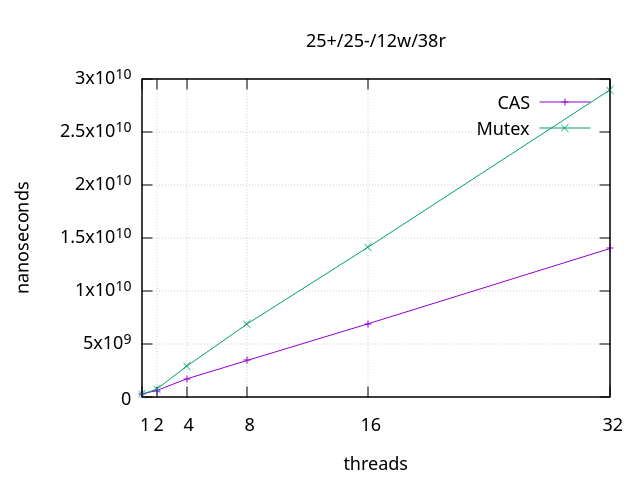
\includegraphics[width=0.5\textwidth]{res1.png}
    \caption{Read Heavy Benchmark of the CAS Vector}
\end{figure}

\begin{figure}[H]
    \centering
    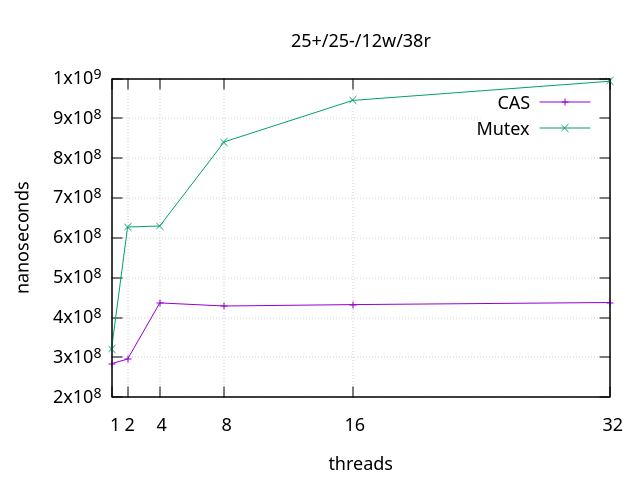
\includegraphics[width=0.5\textwidth]{res2.png}
    \caption{Per Thread Results of the CAS Vector}
\end{figure}
Per Thread results show that CAS implementation is scaling well with the number
of threads.

\subsection{Container Communications: Proposed Design}
To control the bandwidth we used the MemGuard paper \cite{memguard}.
This paper used the performance counters of the intel processor to determine
the read and write access for a physical core in the system. We need to
implement this for a memory region. \\
Performance counters do not provide us with the tracking information for access
to specific memory regions therefore we need to ask either the kernel or
user to do the bookkeeping for the size of the memory access. The user is a better
choice for performance reasons. So our approach is to allocate a budget for each
shared memory region and supplying the user with a library for read and write
purposes. Before every read and write the user will update the bookkeeping
associated with the shared memory region. Also, the budget will be reset on
the hyper-period specified by the real-time system designer. \\
The next goal is to preserve and repurpose the bandwidth. This is done by
predicting the next hyper-period bandwidth usage. This is done using
the exponentially weighted moving average. If our prediction is lower than
the static budget, it will be added to the global bandwidth budget. If a process
needs a budget it can ask the global bandwidth budget for additional budget.
The exact algorithm on how this works can be found in the MemGuard \cite{memguard}
paper. The algorithm used is described as follows:
\begin{algorithm}[h]
    \caption{Memory Bandwidth Reservation Algorithm: Periodic Handler}
    \begin{algorithmic}
        \Begin
            \State $Q_i^{predict} \gets$ output of usage predictor
            \State $Q_i \gets$ user assigned static budget
            \If{$Q_{predict} > Q_i$}
                \State $q_i \gets Q_i$
            \Else
                \State $q_i \gets Q_i^{predict}$
            \EndIf
            \State $G += max\{0,Q_i-q_i\}$
        \End
    \end{algorithmic}
\end{algorithm}
This code gets called on the hyper-period that is defined by the systems
designer.
User-level write and reading must be done by the library provided by us.
Bookkeeping structures live on the first page of the allocated memory that
is unambiguous to the user of the library. Every time a user-level read or write
is called this structure is updated. If a process is over its budget it will
sleep behind the scheduler until the global periodic handler reassigns its
budget. The bookkeeping structure is written as C packed struct as follows:
\begin{lstlisting}[caption= Bookkeeping Struct, frame=tlrb, language=c]
/ *
  * This struct represents the
  * bookkeeping struct that
  * is stored in the first
  * page of the shared memory.
  * This struct is updated by both
  * processes and daemon.
  * /
typedef struct {
    // Allocated Budget
    int read_budget;
    int write_budget;
    int global_budget;
    // Because we need the allocated
    // budget to be unchanged
    // for EWMA
    int read_rem;
    int write_rem;
    // Expected Budget at the start
    int read_ewma;
    int write_ewma;
    // For EWMA calculations
    int it;
} shm_status;
\end{lstlisting}
On the hyper-period, the expected used values are calculated using exponentially
weighted moving averages. According to the MemGuard paper \cite{memguard} this
will help the globally allocated budget aware of the next values and
redistribute unused budget to the process that needs it. \\
Achieving performance isolation in memory is done by bounding the bandwidth.
By bounding the bandwidth we can be sure that no bad or malfunctioning
container creates contention on the system bus and deprive other containers
from using their share of the memory. \\
Bounding the latency can be done using unix signals and
\textit{CLOCK\_THREAD\_CPUTIME\_ID}. If the need arises for such control on
memory we can use it to cancel a read or write function call. This method is
almost unnecessary because most real-time systems designers calculate WCET and
are aware of the communications overhead. \\
Our proposed design is using new kernel system calls to handle creating the
shared memory. Also, shared memory is segmented using a lockless data structure
that eases the uses of mutexes which are bad for real-time scheduling problems.
\begin{figure}[H]
    \centering
    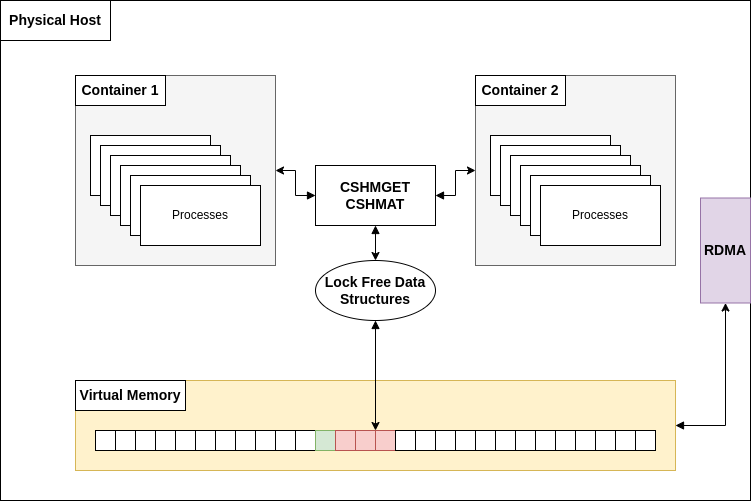
\includegraphics[scale=0.3]{dist.png}
    \caption{Our Proposed Design: Kernel Based}
\end{figure}

\begin{figure}[H]
    \centering
    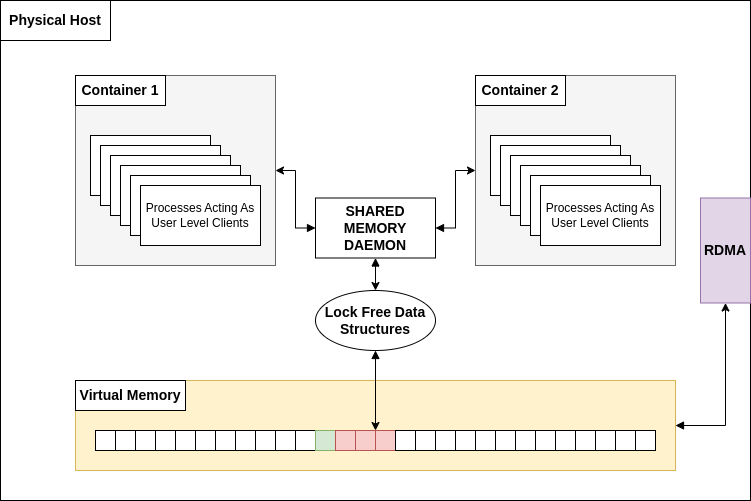
\includegraphics[scale=0.3]{user.png}
    \caption{Our Proposed Design: User Based}
\end{figure}
Our Implementation revolves around the Linux kernel and user-level libraries.
To get shared memory spaces we devised and edited the Linux kernel
and added several syscalls that create and map the address to the
virtual address space of the process. To synchronize the shared memory
between containers we used an atomic vector implementation described in the
\cite{cas}. We implemented the algorithms described in this vector using
compare and swap primitives in the hardware. By having a lock-free
implementation of a synchronized data structure we can be sure that issues
regarding mutexes like priority inversion and hard program verification are
solved in our implementation. \\
Then two programs are written to handle our design goals. One program is a user-level client that is supplied with a user-level bookkeeping library and our
lock-free vector implementation. The other is a server that handles global
budget allocation and hyper-period refreshes. \\
Our results show that the budget is allocated justly and the programs work as
intended. Unfortunately, we could not devise test cases in the allocated
project deadline to show isolation in the presence of a malfunctioning or
bad container.

\section{Conclusion}

In conclusion, this report has explored the importance of inter-process
communication in real-time systems, particularly in the context of virtual
machines and containers. We have discussed the challenges and considerations
involved in designing efficient and deterministic communication methods for
these systems. \\
Shared memory methods, such as shared memory regions, have been identified
as a viable approach for enabling fast and efficient communication between
virtual machines and containers. By leveraging shared memory, we can minimize
the overhead and complexity associated with other communication methods,
such as inter-VM communication. \\
We have also discussed the use of technologies like VirtIO and io\_uring to
optimize the performance of virtual machines and containers.
These technologies provide efficient and low-overhead mechanisms
for I/O operations and system calls, improving the
overall performance of real-time systems. \\
Additionally, we have explored the concept of cache coloring as a technique
to optimize memory performance by reducing cache conflicts.
By carefully assigning memory pages to different cache sets,
we can minimize cache conflicts and improve cache hit rates,
leading to better memory performance. \\
Then we explored lockless shared data structure designs in an attempt to
remove the mutex contention on the shared memory space. We also implemented
a compare and swap vector and compared it to a simple mutex-based vector and
proved that the implementation works as intended.
At last, we tried to propose a design for a shared memory space between the same
host containers and tried to use design ideas from the advanced operating
systems course. \\
The list of achievements is listed as follows:
\begin{itemize}
    \item Proposed and implemented design for a bandwidth-controlled shared
        memory container.
    \item Implemented and benchmarked a lock-free data container for the shared
        memory between processes.
    \item Defined and programmed shared memory system calls inside Linux kernel.
    \item Reviewed the literature on shared memory in virtual machines.
\end{itemize}
Overall, this report highlights the importance of effective and
deterministic communication in real-time systems and provides insights
into various techniques and technologies that can be employed to achieve
this goal. By considering the unique requirements and challenges of
virtual machines and containers, we can design and implement efficient
communication mechanisms that enhance the performance and reliability of
real-time systems in the era of Industry 4.0.

% \bibliographystyle{abbrv}
% \bibliography{references}  % need to put bibtex references in references.bib 

\begin{thebibliography}{10}
    \bibitem{shimmy} Abranches, Marcelo, and Sepideh Goodarzy.
        "Shimmy: Shared memory channels for high performance inter-container
        communication." USENIX Workshop on Hot Topics in Edge Computing
        (HotEdge). 2019.
    \bibitem{mcs}
        Barletta, Marco, et al. "Achieving isolation in mixed-criticality
        industrial edge systems with real-time containers." 34th Euromicro
        Conference on Real-Time Systems (ECRTS 2022). Schloss
        Dagstuhl-Leibniz-Zentrum für Informatik, 2022.
    \bibitem{survey}
        Struhár, Václav, et al. "Real-time containers: A survey."
        2nd Workshop on Fog Computing and the IoT (Fog-IoT 2020).
        Schloss Dagstuhl-Leibniz-Zentrum für Informatik, 2020.
    \bibitem{memguard}
        Yun, Heechul, et al.
        "Memguard: Memory bandwidth reservation system
        for efficient performance isolation in multi-core
        platforms." 2013 IEEE 19th Real-Time and Embedded
        Technology and Applications Symposium (RTAS). IEEE, 2013.
    \bibitem{ordering}
        Adve, Sarita V., and Kourosh Gharachorloo.
        "Shared memory consistency models: A tutorial."
        computer 29.12 (1996): 66-76.
    \bibitem{intel} Intel® 64 Architecture Memory Ordering White Paper
    \bibitem{cas}
        D. Dechev,P. Pirkelbauer, and B. Stroustrup.
        Lock-free Dynamically Resizable Arrays.
        In A. A Shvartsman, editro, OPODIS,
        volume 4305 of Lecture Notes in Computer Science,
        pages 142-156.
        Springer 2006.
    \bibitem{vm}
        Schwäricke, Gero, et al. "A real-time virtio-based framework for
        predictable inter-VM communication." 2021 IEEE Real-Time Systems
        Symposium (RTSS). IEEE, 2021.
\end{thebibliography}
\end{document}
